%%%%%%%%%%%%%%%%%%%%%%%%%%%%%%%%%%%%%%%%%%%%%
%
% 2.1: Delta-Sigma Overview
%
%%%%%%%%%%%%%%%%%%%%%%%%%%%%%%%%%%%%%%%%%%%%%

%%%%%%%%%%%%%%%%%%%%%%%%%%%%%%%%%%%%%%%%%%%%%
%%% 2.1.1 Oversampling
\subsection{Sampling}
The Shannon-Nyquist sampling theorem states that an analog signal must be sampled at a
rate that is equal to at least twice its bandwidth for the analog signal to be
reconstructed from its samples. Specifically, the Shannon-Nyquist sampling theorem
\cite{hayes_schaums_1998} states that if an analog signal, $x_{a}(t)$, is strictly
band-limited, that is,
$$X_{a}(f) = 0 \quad\lvert f\lvert > f_{0}$$
where $X_a(f)$ is the Fourier transform of $x_a(t)$, then $x_a(t)$ can be recovered from
its samples, $x_a(n T_s)$, where $T_s$ is the sampling frequency, if 
%---------------
\begin{equation*}
T_s\leq2f_0
\end{equation*}
%---------------
or equivalently
\begin{equation}\label{eq:nyquist}
  f_{s} = \frac{1}{T_{s}}\geq2f_{0}
\end{equation}
%---------------
where $f_{0}$ is typically referred to as the Nyquist frequency and the minimum sampling
frequency, $2\cdot f_{0}$, is referred to as the Nyquist rate.

Nyquist rate converters are converters which sample the input at the Nyquist
rate of the input signal as given in \eqref{eq:nyquist}. Common implementations of these
include flash, dual-slope, successive approximation (SAR), and pipelined converters
\cite{wikipedia_contributors_analog-to-digital_2007}. In practice, anti-aliasing filter
limitations require Nyquist converters to sample the input at a slightly higher frequency
than the Nyquist rate. Note that current process technologies allow for sample clocks in
the GHz range but limit converter resolution to 16 bits.

%-------------------
\begin{figure}[htbp]
 \centering
 \includegraphics[width=\textwidth]{./final_figures/flash_ADC.eps}
 \caption{Flash ADC System Block Diagram}
 \label{fig:flash_adc}
\end{figure}
%-------------------

In contrast, \DSms belong to a class of systems referred to as oversampling data
converters. Oversampling converters operate at a sampling frequency typically higher than 
Nyquist rate converters. However, the operational bandwidth of the \DSm is a fraction
of the sampling frequency \cite{johns_analog_1996}\cite{oppenheim_discrete-time_1999}.
The ratio of the sampling frequency to the operational bandwidth is referred to as
the oversampling-rate (OSR) which is defined as
%---------------
\begin{equation}
 \textrm{OSR}=\frac{f_{s}}{2f_{0}}
\end{equation}
%---------------
where $f_{0}$ and $f_{s}$ correspond to the Nyquist and sampling frequency respectively.
There is a finite amount of performance increase to be had from increasing the OSR. Thus,
in practice, OSRs between 8 and 256 are often used.

%%%%%%%%%%%%%%%%%%%%%%%%%%%%%%%%%%%%%%%%%%%%
%%% 2.1.2 Quantization Noise

\subsection{Quantization Noise}
Quantization is defined as the process by which a theoretically infinite precision signal
is approximated by one of a finite number of fixed levels referred to as quantization
levels. This process is a nonlinear transformation that can be modeled linearly as
additive white noise. To illustrate, consider an analog signal, $x_a(t)$, and its
corresponding discrete signal $x(n)$. If $x(n)$ is a $B+1$ bit signal such that 
\begin{equation*}
\bigl|x(n)\bigr| \leq X_m2^B 
\end{equation*}
%---------------
where $X_m$ represents the full-scale signal amplitude, the number of quantization
levels, $L$, is given as
%---------------
\begin{equation}\label{eq:quantization_bits}
 L=2^{B+1}\text{.}
\end{equation}
%---------------
If the quantization interval, $\Delta$, can be further defined as the distance between
any two adjacent quantization levels and is given as
%---------------
\begin{equation}\label{eq:quantization_delta}
 \Delta=\frac{X_m}{2^B}
\end{equation}
%---------------
where $X_m$ and $B$ correspond the full-scale signal amplitude and number of bits
available to represent the signal. To avoid saturating the quantizer, the quantizer input
is typically normalized with respect to the full-scale quantizer input range, $X_m$,
which reduces \eqref{eq:quantization_delta} to $2^{-B}$ illustrating that the grain of the
quantizer is largely determined by the number of quantization bits available. However,
even for a large number of bits, the quantizer output is still a coarse approximation of
its input.

%-------------------
\begin{figure}[htbp]
 \centering
 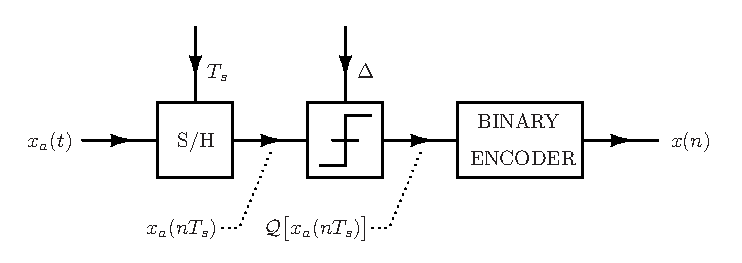
\includegraphics{./final_figures/basic_ADC.eps}
 \caption{Basic ADC Block Diagram}
 \label{fig:basic_adc}
\end{figure}
%-------------------

The difference between the sampled input, $x(nT_s)$, and the quantizer output,
$\hat{x}(n)$, at each interval is referred to as the quantization error. The
quantizer output is expressed as the sum of the sampled input signal, $x(n)$, and the
quantization error, $e(n)$, at each interval as given by
%---------------
\begin{equation}\label{eq:quantizer_output}
\hat{x}(n)=\mathcal{Q}\left[x(n)\right]=x(n T_s)+e(n)
\end{equation}
%---------------
where $\mathcal{Q}[\cdot] $ represents the nonlinear quantization process.
Modeling the quantization error as given in \eqref{eq:quantizer_output} eases the
mathematical complexity of the quantization process. Specifically, $e(n)$ is modeled as 
a uniformly distributed noise source that is uncorrelated with $x(n)$ and all other
noise sources. As such, we will also make the following assumptions
\cite{gray_quantization_1990}\cite{oppenheim_discrete-time_1999}:
%---------------
\begin{itemize}
 \item $e(n)$ is a stationary random process
 \item $e(n)$ is uncorrelated with the quantizer input $x(n)$
 \item samples (random variables of the random process) of $e(n)$ are uncorrelated
thereby making it a white-noise process
 \item the distribution of the random error process is uniform over the quantization
error range $\left[-\frac{\Delta}{2},\frac{\Delta}{2}\right]$
\end{itemize}

Modeling the quantization error as an additive white noise source allows for the \DSm to
be modeled as a two-input / one-output linear system as given by
%---------------
\begin{equation}\label{eq:DSM_output_1}
 y(n)=\mathcal{T}_s[x(n)]+\mathcal{T}_n[e(n)]
\end{equation}
%---------------
where $x(n)$ and $y(n)$ correspond to the discrete time system input and output
respectively, $\mathcal{T}_s[\cdot]$ represents the transformation of the input
signal, $x(n)$, and $\mathcal{T}_n[\cdot]$ is the transformation of the noise signal,
$e(n)$. Note that $\mathcal{T}_s[\cdot]$ and $\mathcal{T}_n[\cdot]$ illustrate the
conditioning of the input signal and the noise respectively. The conditioning of the
independent noise source is referred to as noise shaping and will be addressed in the next
section.

%%%%%%%%%%%%%%%%%%%%%%%%%%%%%%%%%%%%%%%%%%%%
%%% 2.1.3 Noise-Shaping

\subsection{Noise-Shaping}
As discussed in the previous section, the output, $y(n)$, of a \DSm can be written as
given in \eqref{eq:DSM_output_1}. Because the noise transformation,
$\mathcal{T}_n[\cdot]$ (NTF), is different from the signal transformation,
$\mathcal{T}_s[\cdot]$ (STF), the quantization noise can be shaped or filtered
differently than the input signal. Such systems are referred to as noise-shaping systems.

In \DSms, noise shaping is achieved by adding a negative feedback path from the quantizer
output to the loop filter input as illustrated in Figure \ref{fig:loop_filter_1}. 
%-------------------
\begin{figure}[htbp]
 \centering
 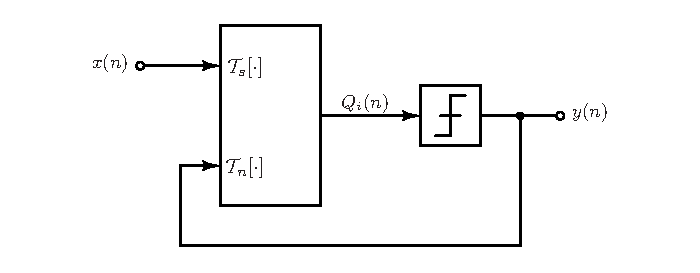
\includegraphics{./final_figures/loop_filter.eps}
 \caption{Noise Shaping \DSM Block Diagram}
 \label{fig:loop_filter_1}
\end{figure}
%-------------------
It follows that employing classical filter design techniques allows for the
composite system to be frequency selective. Thus, \DSms are referred to as
\textit{low-pass} or \textit{band-pass} respective of how the noise shaping occurs. Figure
\ref{fig:noise_shaping_spectrum} illustrates an example low-pass \DSm system.
%-------------------
\begin{figure}[htbp]
 \centering
 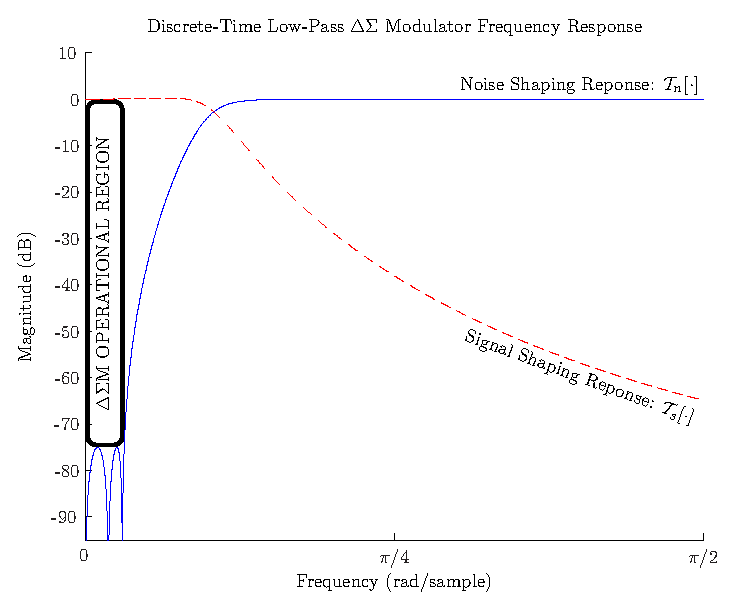
\includegraphics{./final_figures/DSM_noise_shaping_ex_final.eps}
 \caption{\DSM Frequency Response Example}
 \label{fig:noise_shaping_spectrum}
\end{figure}
%-------------------
Note that the conditioning of the input signal is complementary to the shaping of the
noise. Also, note that the input signal is unity within the region denoted as the
$\Delta\Sigma$M operational region while the noise is heavily attenuated. These
characteristics are precisely what define \DSms from a global system perspective and will
be addressed fully in the following sections.
